\section{Questão 166 - Geometria, Pitágoras, Radicais}

Construir figuras de diversos tipos, apenas dobrando e cortando papel, sem cola e sem tesoura, é a arte do origami (ori = dobrar; kami = papel), que tem um significado altamente simbólico no Japão. A base do origami é o conhecimento do mundo por base do tato. Uma jovem resolveu construir um cisne usando a técnica do origami, utilizando uma folha de papel de 18 cm por 12 cm. Assim, começou por dobrar a folha conforme a figura.

\begin{figure}[H]
    \centering
    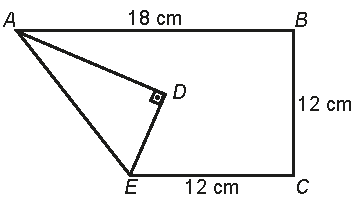
\includegraphics[width=0.95\linewidth]{Q166.pdf}
    %\caption{}
    \label{fig:q166}
\end{figure}

Após essa primeira dobradura, a medida do segmento AE é

A) $ 2\sqrt{22} cm $.

B) $ 6\sqrt{3} cm $.

C) $ 12 cm $.

D) $ 6\sqrt{5} cm $.

E) $ 12\sqrt{2} cm $.

\textbf{Resolução}

É muito óbvio a aplicação direta do Teorema de Pitágoras:



\tikzset{every picture/.style={line width=2pt}} %set default line width to 0.75pt        

\noindent \resizebox{.5\textwidth}{!}{
    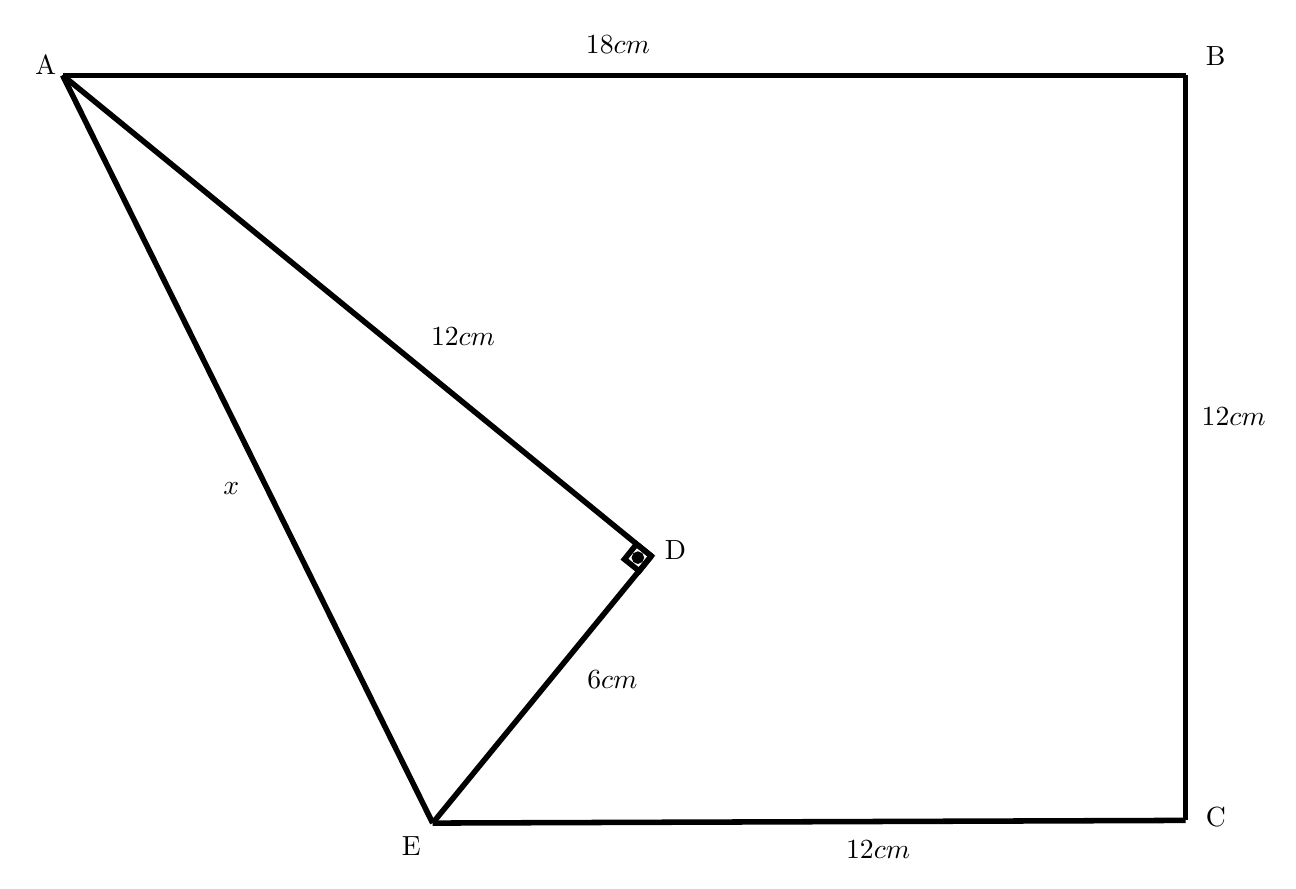
\begin{tikzpicture}[x=0.75pt,y=0.75pt,yscale=-1,xscale=1]
    %uncomment if require: \path (0,473); %set diagram left start at 0, and has height of 473
    
    %Straight Lines [id:da7181388705522671] 
    \draw    (61.5,31) -- (602.5,31) ;
    %Straight Lines [id:da44939859555890327] 
    \draw    (602.5,31) -- (602.5,390) ;
    %Straight Lines [id:da1206829123410158] 
    \draw    (239.8,391.29) -- (602.5,390) ;
    %Straight Lines [id:da15071438547047888] 
    \draw    (61.5,31) -- (239.8,391.29) ;
    %Straight Lines [id:da24551929708671127] 
    \draw    (345.13,262.63) -- (239.8,391.29) ;
    %Straight Lines [id:da6934731152853295] 
    \draw    (61.5,31) -- (345.13,262.63) ;
    %Shape: Rectangle [id:dp45624327686007016] 
    \draw   (338,256.91) -- (345.13,262.63) -- (339.32,269.88) -- (332.18,264.16) -- cycle ;
    %Shape: Circle [id:dp7419514115799553] 
    \draw  [fill={rgb, 255:red, 0; green, 0; blue, 0 }  ,fill opacity=1 ] (337.06,263.39) .. controls (337.06,262.51) and (337.78,261.8) .. (338.66,261.8) .. controls (339.54,261.8) and (340.25,262.51) .. (340.25,263.39) .. controls (340.25,264.27) and (339.54,264.99) .. (338.66,264.99) .. controls (337.78,264.99) and (337.06,264.27) .. (337.06,263.39) -- cycle ;
    
    % Text Node
    \draw (46,19.33) node [anchor=north west][inner sep=0.75pt]   [align=left] {A};
    % Text Node
    \draw (610,14.67) node [anchor=north west][inner sep=0.75pt]   [align=left] {B};
    % Text Node
    \draw (610,381.33) node [anchor=north west][inner sep=0.75pt]   [align=left] {C};
    % Text Node
    \draw (349.33,252.67) node [anchor=north west][inner sep=0.75pt]   [align=left] {D};
    % Text Node
    \draw (222.67,395.33) node [anchor=north west][inner sep=0.75pt]   [align=left] {E};
    % Text Node
    \draw (311.33,9.4) node [anchor=north west][inner sep=0.75pt]    {$18cm$};
    % Text Node
    \draw (608,188.73) node [anchor=north west][inner sep=0.75pt]    {$12cm$};
    % Text Node
    \draw (436.67,397.4) node [anchor=north west][inner sep=0.75pt]    {$12cm$};
    % Text Node
    \draw (312,315.4) node [anchor=north west][inner sep=0.75pt]    {$6cm$};
    % Text Node
    \draw (236.67,150.07) node [anchor=north west][inner sep=0.75pt]    {$12cm$};
    % Text Node
    \draw (136.67,224.73) node [anchor=north west][inner sep=0.75pt]    {$x$};
    
    
    \end{tikzpicture}
}

\textbf{Rascunho}

\opmul[decimalsepsymbol={,},displayintermediary=all]{1.01}{1.01}\flexquad{3}
\opdiv[decimalsepsymbol={,},displayintermediary=all]{202}{1.01}\flexquad{3}
\opset{strikedecimalsepsymbol={\rlap{,}\rule[-1pt]{3pt}{0.4pt}}}
\opdiv[decimalsepsymbol={,},shiftdecimalsep=both,displayintermediary=all]{204.02}{1.0201}\quad


\begin{center}
    \href{https://youtu.be/}{
        \qrcode{https://youtu.be/}
    }\\
    Resolução: \url{https://youtu.be/}
\end{center}
